\documentclass[12pt,a4paper]{article}

\usepackage{fontspec}
\usepackage{xeCJK}
\usepackage{graphicx}
\usepackage[normalem]{ulem}
\usepackage{geometry}
\usepackage{hyperref}

\geometry{a4paper,margin=2.5cm}

\setmainfont{TeX Gyre Termes}
\setCJKmainfont{Noto Serif CJK SC}

\newcommand{\ul}[1]{\underline{#1}}

\begin{document}

\textbf{《系统开发工具基础》实验报告}

\textbf{姓 名：} \ul{夏昕}

\textbf{学 号：} \ul{25080012068}

\textbf{专 业：} \ul{软件工程}

\textbf{实验时间：} \ul{2026/8/24}

\textbf{任课教师：} \ul{周小伟}

\textbf{commit记录}

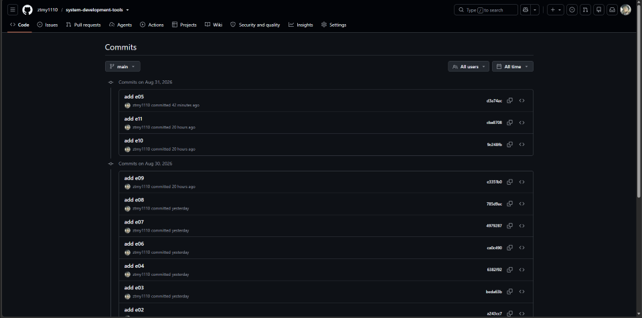
\includegraphics[width=6.65354in,height=3.8132in]{media/media/image1.png}

\textbf{课堂习题}

\textbf{第1题：含空格文件名的批量整理}

\textbf{一、主题}

Shell 基础与文件系统

\textbf{二、题目要求}

1.创建input/docs 和 input/tmp；创建 input/docs/notes
one.txt（内容为alpha和beta两行）、input/docs/.secret.txt（内容为
hidden）、input/tmp/empty.txt（空文件）以及
input/run.log（任意两行日志）。

2.显示q01的绝对路径，并以长格式列出input下全部项目，包含隐藏文件。

3.把input下所有.txt文件复制到work/\textless 学号\textgreater/，保留相对目录结构并正确处理名称中的空格。

4.将复制后的目录权限设为750、普通文件权限设为640；生成inventory.txt，列出相对路径和字节数。

\textbf{三、源程序代码}

cd \textasciitilde/Epi1

mkdir -p q01

cd q01

mkdir -p input/docs input/tmp

echo -e "alpha\textbackslash nbeta" \textgreater{} "input/docs/notes
one.txt"

echo "hidden" \textgreater{} "input/docs/.secret.txt"

touch "input/tmp/empty.txt"

echo -e "log line 1\textbackslash nlog line 2" \textgreater{}
input/run.log

pwd

ls -laR input

mkdir -p "work/25080012068/docs"

mkdir -p "work/25080012068/tmp"

find input/docs -type f -name "*.txt" -exec cp \{\}
"work/25080012068/docs/" \textbackslash;

find input/tmp -type f -name "*.txt" -exec cp \{\}
"work/25080012068/tmp/" \textbackslash;

find "work/25080012068" -type d -exec chmod 750 \{\} \textbackslash;

find "work/25080012068" -type f -exec chmod 640 \{\} \textbackslash;

find "work/25080012068" -type f -printf \textquotesingle\%P \%s
bytes\textbackslash n\textquotesingle{} \textgreater{} inventory.txt

cat inventory.txt

\textbf{四、程序运行结果}

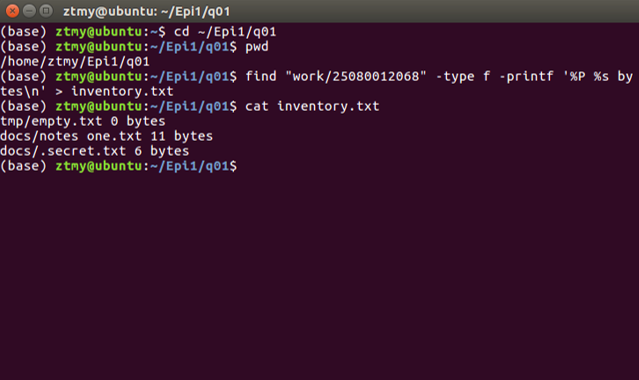
\includegraphics[width=6.65694in,height=3.95556in]{media/media/image2.png}

\textbf{五、解题感悟}

1. 熟悉了 mkdir、cp、find、chmod 等常用 Shell 命令。

2. 认识到处理带空格和隐藏文件时需要注意路径和文件名的写法。

3. 对 Linux 文件权限以及命令行批量处理文件有了更直观的理解。

\textbf{第2题：随机访问日志统计}

\textbf{一、主题}

Shell 管道与文本处理

\textbf{二、题目要求}

1.编写analyze.sh，接收一个CSV文件路径；文件不存在时将错误写入stderr并返回非零退出码。

2.使用Shell管道以及awk、sort、head等工具，输出HTTP5xx数量最多的前2个path；按次数降序，次数相同时按path字典序。

3.输出全部数据行的平均latency\_ms，保留两位小数；表头不得计入。

4.分别对access.csv和一个不存在的文件运行脚本；不得使用Python、电子表格或手工统计。

\textbf{三、源程序代码}

cd \textasciitilde/Epi1/q02

touch access.csv analyze.sh

vim access.csv

vim analyze.sh

./analyze.sh access.csv

./analyze.sh test.csv

\textbf{\ul{analyze.sh}}

\#!/bin/bash

if {[} \$\# -ne 1 {]}; then

echo "Usage: \$0 \textless csv\_file\textgreater" \textgreater\&2

exit 1

fi

if {[} ! -f "\$1" {]}; then

echo "Error: file \textquotesingle\$1\textquotesingle{} does not exist"
\textgreater\&2

exit 1

fi

echo "Top 2 HTTP 5xx paths:"

awk -F, \textquotesingle{}

NR \textgreater{} 1 \&\& \$4 \textgreater= 500 \&\& \$4 \textless{} 600
\{

count{[}\$3{]}++

\}

END \{

for (path in count) \{

print path, count{[}path{]}

\}

\}

\textquotesingle{} "\$1" \textbar{}

sort -k2,2nr -k1,1 \textbar{}

head -2

echo "Average latency\_ms:"

awk -F, \textquotesingle{}

NR \textgreater{} 1 \{

sum += \$5

count++

\}

END \{

printf "\%.2f\textbackslash n", sum / count

\}

\textquotesingle{} "\$1"

\textbf{四、程序运行结果}

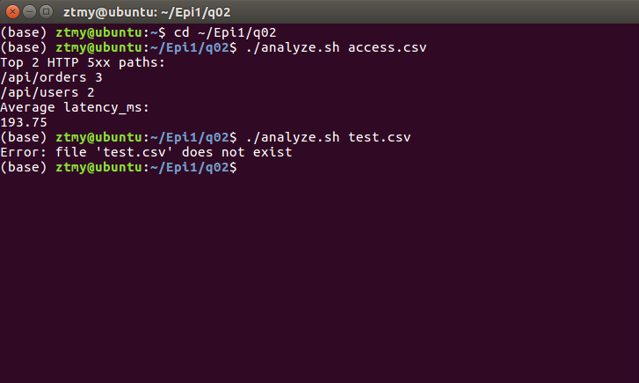
\includegraphics[width=6.65694in,height=3.98542in]{media/media/image3.png}

\textbf{五、解题感悟}

1. 熟悉了 awk、sort、head 以及管道的基本使用方法。

2. 学会了通过多个 Shell 命令组合完成 CSV 数据统计。

3. 加深了对 Shell 脚本、错误处理和管道处理思想的理解。

\textbf{第3题：制造、解决并解释一次合并冲突}

\textbf{一、主题}

Version Control and Git

\textbf{二、题目要求}

1.初始化仓库，在main创建config.txt，内容为mode=normal，并完成初始提交。

2.创建feature-a，把内容改为mode=safe并提交；从初始main创建feature-b，把内容改为mode=fast并提交。

3.回到main，先合并feature-a，再合并feature-b；解决冲突时保留mode=safe，并另加一行

note=reviewed。

4.确认工作区干净，运行gitlog --all --graph --decorate -\/-oneline
查看历史。

\textbf{三、源程序代码}

cd \textasciitilde/Epi1

mkdir -p q03

cd q03

git init

echo "mode=normal" \textgreater{} config.txt

git add config.txt

git commit -m "Initial commit"

git branch -M main

git checkout -b feature-a

echo "mode=safe" \textgreater{} config.txt

git add config.txt

git commit -m "Set mode to safe"

git checkout main

git checkout -b feature-b

echo "mode=fast" \textgreater{} config.txt

git add config.txt

git commit -m "Set mode to fast"

git checkout main

git merge feature-a

git merge feature-b

printf "mode=safe\textbackslash nnote=reviewed\textbackslash n"
\textgreater{} config.txt

git add config.txt

git commit -m "Resolve merge conflict"

git status

git log -\/-all -\/-graph -\/-decorate -\/-oneline

cat config.txt

\textbf{四、程序运行结果}

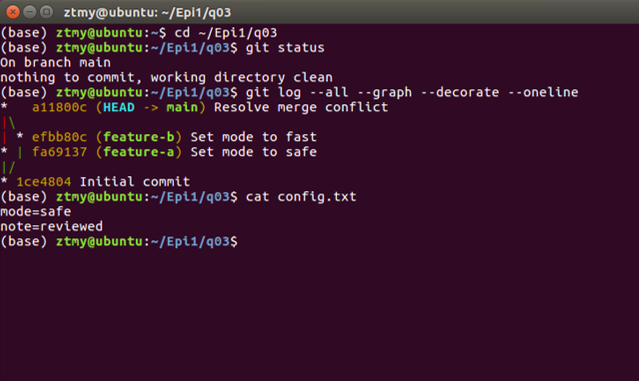
\includegraphics[width=6.65694in,height=3.97014in]{media/media/image4.png}

\textbf{五、解题感悟}

1. 进一步理解了 Git 中分支、提交和合并的基本概念。

2. 通过实际操作认识了合并冲突产生的原因以及解决方法。

3. 对 Git 的版本管理和分支协作流程有了更加清晰的认识。

\textbf{第4题：修复并构建一页技术说明}

\textbf{一、主题}

LaTeX 文档编辑

\textbf{二、题目要求}

1.加入一个带编号和label的公式，并在正文中使用ref或eqref引用。

2.加入一个2行2列表格，设置caption和label，并在正文中引用该表。

3.使用latexmk-pdf-halt-on-error 或 tectonic 生成 report.pdf。

4.确认PDF能打开，且交叉引用不显示``??''。

\textbf{三、源程序代码}

cd \textasciitilde/Epi1

mkdir -p q04

cd q04

vim report.tex

latexmk -pdf -halt-on-error report.tex

ls -lh

xdg-open report.pdf

\textbf{\ul{report.tex}}

\textbackslash documentclass\{article\}

\textbackslash usepackage\{amsmath\}

\textbackslash begin\{document\}

\textbackslash title\{Tool Report\}

\textbackslash author\{Xia Xin-25080012068\}

\textbackslash maketitle

\textbackslash section\{Result\}

This experiment demonstrates the use of Git and LaTeX tools.

The following equation describes the relationship between energy,

mass, and the speed of light:

\textbackslash begin\{equation\}

E = mc\^{}2

\textbackslash label\{eq:energy\}

\textbackslash end\{equation\}

As shown in Equation\textasciitilde\textbackslash eqref\{eq:energy\},
\$E\$ represents energy,

\$m\$ represents mass, and \$c\$ represents the speed of light in
vacuum.

The experimental results are shown in
Table\textasciitilde\textbackslash ref\{tab:result\}.

\textbackslash begin\{table\}{[}htbp{]}

\textbackslash centering

\textbackslash caption\{Tool Experiment Results\}

\textbackslash label\{tab:result\}

\textbackslash begin\{tabular\}\{cc\}

\textbackslash hline

Tool \& Result \textbackslash\textbackslash{}

\textbackslash hline

Git \& Pass \textbackslash\textbackslash{}

LaTeX \& Pass \textbackslash\textbackslash{}

\textbackslash hline

\textbackslash end\{tabular\}

\textbackslash end\{table\}

As shown in Table\textasciitilde\textbackslash ref\{tab:result\}, both
Git and LaTeX operations

were completed successfully.

\textbackslash end\{document\}

\textbf{四、程序运行结果}

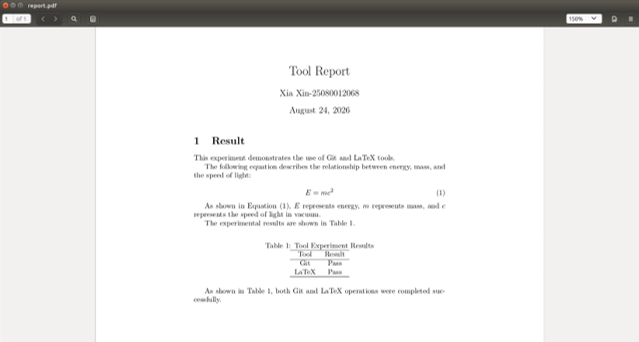
\includegraphics[width=6.65694in,height=3.56736in]{media/media/image5.png}

\textbf{五、解题感悟}

1. 熟悉了 LaTeX 文档的基本结构以及命令行编译方法。

2. 学会了使用 label、ref 和 eqref 实现公式和表格的交叉引用。

3. 加深了对 LaTeX 技术文档排版和 PDF 生成流程的理解。

\textbf{课后练习}

\textbf{练习1：脚本编写与文件读取}

\textbf{一、主题}

Shell 基础与文件系统

\textbf{二、题目要求}

写一个脚本，接收文件名参数（\$1），用 test -f 或 {[} -f ... {]}
检查该文件是否存在，并根据结果输出不同提示。

\textbf{三、源程序代码}

\textbf{\ul{check.sh}}

\#!/bin/bash

if {[} -f "\$1" {]};then

echo "file exists: \$1"

else

echo "file not found: \$1"

fi

\textbf{四、程序运行结果}

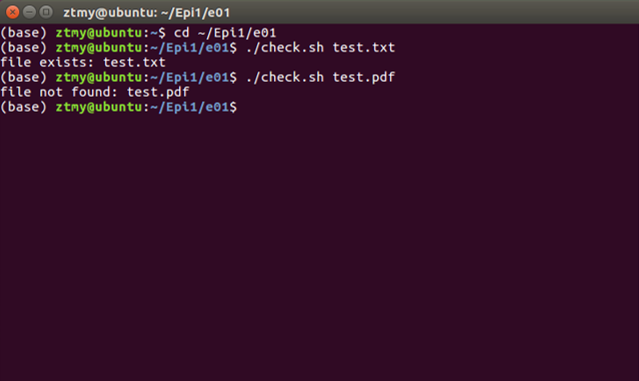
\includegraphics[width=6.65694in,height=3.97014in]{media/media/image6.png}

\textbf{五、解题感悟}

1. 学会了使用 `\$1` 获取脚本运行时传入的文件名参数。

2. 熟悉了 `test -f` 和 `{[} -f ... {]}` 判断文件是否存在的方法。

3. 加深了对 Shell 中条件判断和分支结构的理解。

\textbf{练习2：shell的标准流与重定向}

\textbf{一、主题}

Shell 基础与文件系统

\textbf{二、题目要求}

Shell 有三条标准流：stdin（0）、stdout（1）、stderr（2）。运行 ls
/nonexistent /tmp ，把 stdout 和 stderr
分别重定向到两个文件。你将如何把两者都重定向到同一个文件？

\textbf{三、源程序代码}

cd Epi1/e02

touch stdout.txt stderr.txt

ls /nonexistent /tmp \textgreater{} stdout.txt 2\textgreater{}
stderr.txt

cat stdout.txt stderr.txt

touch output.txt

ls /nonexistent /tmp \textgreater{} output.txt 2\textgreater\&1

cat output.txt

\textbf{四、程序运行结果}

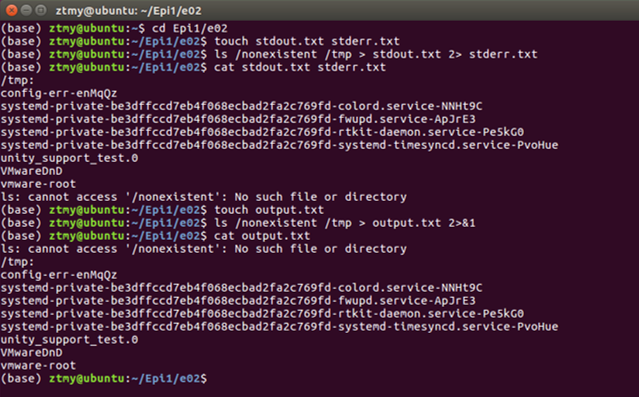
\includegraphics[width=6.65694in,height=4.13403in]{media/media/image7.png}

\textbf{五、解题感悟}

1. 了解了 Shell 中 stdin、stdout 和 stderr 三种标准流及其文件描述符。

2. 学会了使用 `\textgreater` 和 `2\textgreater`
分别重定向标准输出和标准错误。

3. 理解了 `2\textgreater\&1`
的作用，掌握了将标准输出和错误输出合并到同一文件的方法。

\textbf{练习3：条件执行与退出状态控制}

\textbf{一、主题}

Shell 基础与文件系统

\textbf{二、题目要求}

\$? 保存上一条命令的退出状态（0 表示成功）。\&\&
仅在前一条成功时执行后一条；\textbar\textbar{}
仅在前一条失败时执行后一条。写一个一行命令：仅当 /tmp/mydir
不存在时才创建它。

\textbf{三、源程序代码}

test -d /tmp/mydir \textbar\textbar{} mkdir -p /tmp/mydir

\textbf{四、程序运行结果}

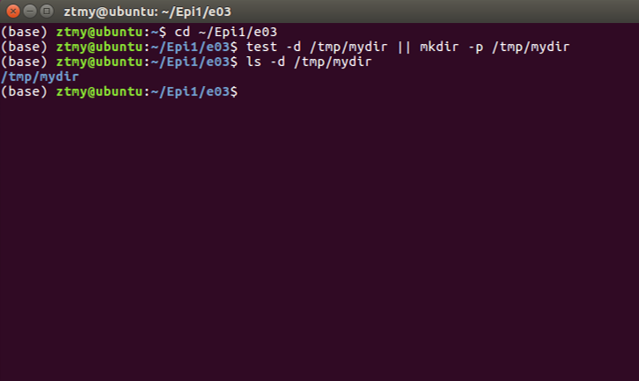
\includegraphics[width=6.65694in,height=3.97014in]{media/media/image8.png}

\textbf{五、解题感悟}

1. 学会了使用 \textbar\textbar{}
根据上一条命令的执行结果决定是否执行后续命令。

2. 进一步理解了 `/tmp`、`\textasciitilde` 和 `./`
的区别，能够区分绝对路径和相对路径。

3. 通过实际操作发现，Shell
命令比较简单，但路径写错或者符号使用错误就容易导致命令执行失败。

\textbf{练习4：命令替换与日期格式化}

\textbf{一、主题}

Shell 基础与文件系统

\textbf{二、题目要求}

写一条命令，把文件复制为带当天日期的备份文件名（例如 notes.txt →
notes\_2026-01-12.txt）。（提示：\$(date +\%Y-\%m-\%d)）

\textbf{三、源程序代码}

cp notes.txt "notes\_\$(date +\%Y-\%m-\%d).txt"

\textbf{四、程序运行结果}

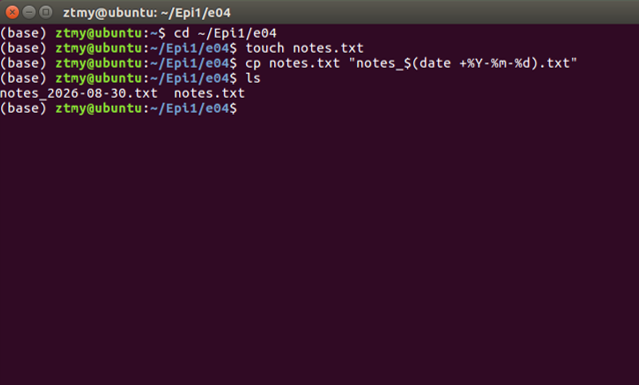
\includegraphics[width=6.65694in,height=4.01458in]{media/media/image9.png}

\textbf{五、解题感悟}

1. 学会了使用 `\$(...)` 进行命令替换，将 `date`
命令的结果直接用于文件名。

2. 进一步理解了 `\%Y`、`\%m`、`\%d`
等日期格式符号的含义，可以按照指定格式获取当前日期。

3.
通过实际操作掌握了利用当前日期生成备份文件名的方法，也认识到命令替换在
Shell 中可以提高命令使用的灵活性。

\textbf{练习5：}

\textbf{一、主题}

Shell 管道与文本处理

\textbf{二、题目要求}

使用管道找出你「home 目录」中最常见的 5 种文件扩展名。（提示：组合 find
、grep / sed / awk、sort、uniq -c 以及 head）

\textbf{三、源程序代码}

find \textasciitilde{} -type f \textbar{} sed
\textquotesingle s/.*\textbackslash.//\textquotesingle{} \textbar{} grep
-v \textquotesingle/\textquotesingle{} \textbar{} sort \textbar{} uniq
-c \textbar{} sort -nr \textbar{} head -5

\textbf{四、程序运行结果}

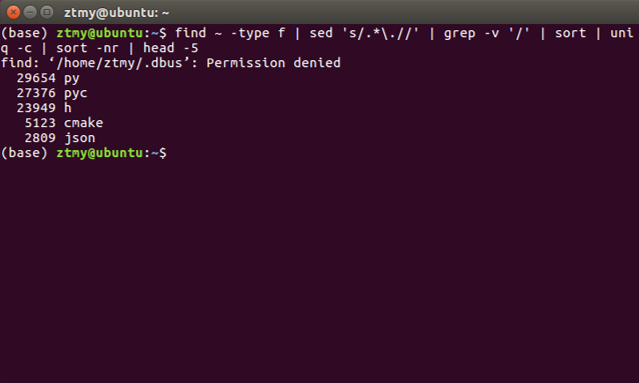
\includegraphics[width=6.65694in,height=3.98542in]{media/media/image10.png}

\textbf{五、解题感悟}

1. 学会了使用 `find`
查找文件，并通过管道把多个命令连接起来完成文件扩展名统计。

2. 进一步理解了 `sed`、`sort`、`uniq -c` 和 `head`
的作用，特别是学会了用 `sed` 提取文件扩展名。

3.
通过这道题发现，多个简单命令组合起来也能完成比较复杂的任务，对管道的使用更加熟悉了。

\textbf{练习6：使用 find、xargs 统计 Shell 文件行数}

\textbf{一、主题}

Shell 管道与文本处理

\textbf{二、题目要求}

1.xargs 会把 stdin 的每一行转换为命令参数。

2.结合 find 和 xargs（不要用 find -exec），找出目录中所有 .sh 文件，并用
wc -l 统计每个文件行数。

3.加分项：正确处理文件名中的空格。（提示：-print0 和 -0）

\textbf{三、源程序代码}

find .. -type f -name "*.sh" -print0 \textbar{} xargs -0 -n 1 wc -l

\textbf{四、程序运行结果}

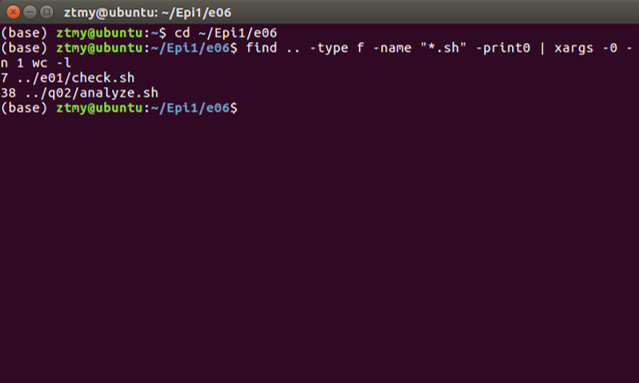
\includegraphics[width=6.65694in,height=3.98542in]{media/media/image11.png}

\textbf{五、解题感悟}

1. 学会了使用 `find` 查找指定类型的文件，并通过管道将结果传给 `xargs`
继续处理。

2. 进一步理解了 `-print0` 和 `-0`
的作用，能够正确处理文件名中包含空格的情况。

3. 通过这道题熟悉了 `wc -l` 的用法，也更加理解了多个 Shell
命令通过管道组合使用的方法。

\textbf{练习7：使用 git stash 暂存未提交的修改}

\textbf{一、主题}

Version Control and Git

\textbf{二、题目要求}

1.Clone 一个 GitHub 仓库，修改其中一个已有文件，然后执行 git
stash，观察工作区变化。

2.运行 git log -\/-all -\/-oneline 查看历史。

3.再运行 git stash pop 恢复修改，并说明 git stash 在什么场景下有用。

\textbf{三、源程序代码}

cd \textasciitilde/Epi1

git clone \url{https://github.com/octocat/Hello-World.git}

cd Hello-World

ls

echo "test change" \textgreater\textgreater{} README

git status

git stash

git status

git log -\/-all -\/-oneline

git stash pop

git status

\textbf{四、程序运行结果}

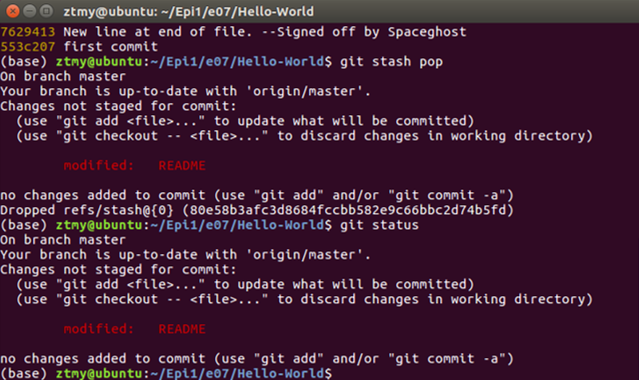
\includegraphics[width=6.65694in,height=3.95556in]{media/media/image12.png}

\textbf{五、解题感悟}

1. 学会了使用 `git stash` 临时保存没有提交的修改，并通过 `git stash pop`
将修改恢复回来。

2. 通过实际操作了解了 `git stash` 和 `git commit` 的区别，知道 stash
保存的是临时修改，不会直接形成普通提交记录。

3. 通过这道题认识到，在需要临时切换分支或者处理其他任务时，可以使用 `git
stash` 保存当前工作，避免未完成的修改影响后续操作。

\textbf{练习8：使用 git config 创建命令别名}

\textbf{一、主题}

Version Control and Git

\textbf{二、题目要求}

1.和许多命令行工具一样，Git 也提供了一个配置文件（也叫
dotfile，隐藏配置文件），名为 \textasciitilde/.gitconfig。

2.请在 \textasciitilde/.gitconfig 中创建一个别名，使得运行 git graph
时，可以得到 git log -\/-all -\/-graph -\/-decorate -\/-oneline 的输出。

3.你可以直接编辑 \textasciitilde/.gitconfig 文件，也可以使用 git config
命令来添加别名。

\textbf{三、源程序代码}

git config -\/-global alias.graph \textquotesingle log -\/-all -\/-graph
-\/-decorate -\/-oneline\textquotesingle{}

\textbf{四、程序运行结果}

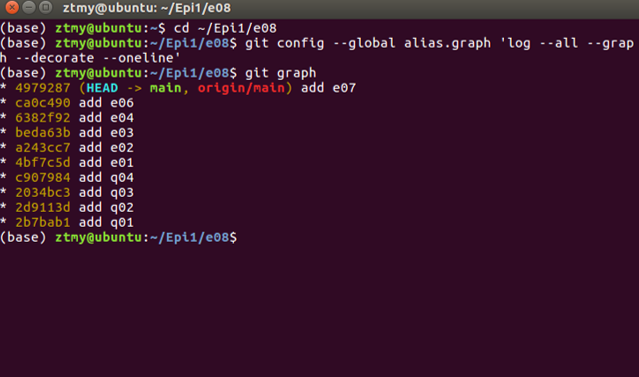
\includegraphics[width=6.65694in,height=3.92569in]{media/media/image13.png}

\textbf{五、解题感悟}

1. 学会了使用 `git config` 配置 Git
别名，可以用简单的命令代替较长的命令。

2. 进一步了解了 `\textasciitilde/.gitconfig`
文件的作用，知道它可以保存当前用户的 Git 配置。

3. 通过这道题认识到给常用命令设置别名可以减少重复输入，提高使用 Git
的效率。

\textbf{练习9：LaTeX 表格的创建与编译}

\textbf{一、主题}

LaTeX 文档编辑

\textbf{二、题目要求}

尝试画出下列表格：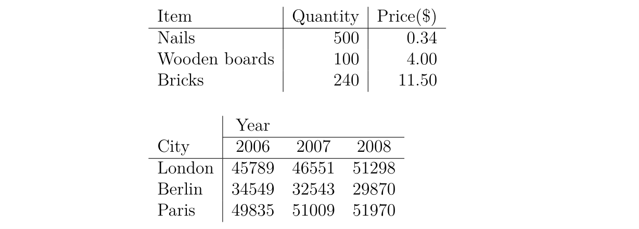
\includegraphics[width=6.65694in,height=2.38819in]{media/media/image14.png}

\textbf{三、源程序代码}

cd \textasciitilde/Epi1/e09

touch table.tex

vim table.tex

latexmk -pdf table.tex

xdg-open table.pdf

\textbf{\ul{table.tex}}

\textbackslash documentclass\{article\}

\textbackslash begin\{document\}

\textbackslash begin\{tabular\}\{l\textbar r\textbar r\}

\textbackslash hline

Item \& Quantity \& Price(\textbackslash\$)
\textbackslash\textbackslash{}

\textbackslash hline

Nails \& 500 \& 0.34 \textbackslash\textbackslash{}

Wooden boards \& 100 \& 4.00 \textbackslash\textbackslash{}

Bricks \& 240 \& 11.50 \textbackslash\textbackslash{}

\textbackslash end\{tabular\}

\textbackslash vspace\{1cm\}

\textbackslash begin\{tabular\}\{l\textbar r\textbar r\textbar r\}

\textbackslash hline

City \& \textbackslash multicolumn\{3\}\{c\}\{Year\}
\textbackslash\textbackslash{}

\textbackslash cline\{2-4\}

\& 2006 \& 2007 \& 2008 \textbackslash\textbackslash{}

\textbackslash hline

London \& 45789 \& 46551 \& 51298 \textbackslash\textbackslash{}

Berlin \& 34549 \& 32543 \& 29870 \textbackslash\textbackslash{}

Paris \& 49835 \& 51009 \& 51970 \textbackslash\textbackslash{}

\textbackslash end\{tabular\}

\textbackslash end\{document\}

\textbf{四、程序运行结果}

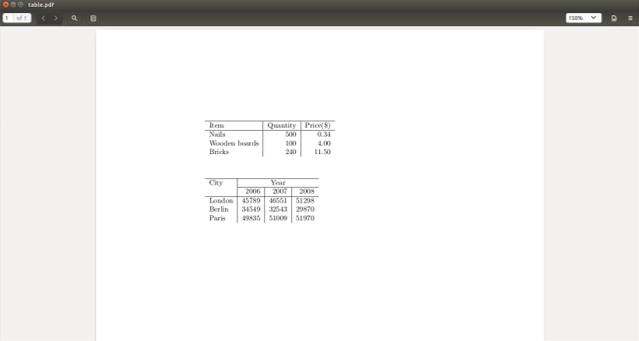
\includegraphics[width=6.65694in,height=3.55208in]{media/media/image15.png}

\textbf{五、解题感悟}

1. 学会了使用 `tabular` 环境创建 LaTeX 表格，并了解了
`\&`、`\textbackslash\textbackslash` 和 `\textbackslash hline`
的基本用法。

2. 通过编译过程中出现的报错，发现 LaTeX
对命令拼写要求比较严格，一个字母写错也可能产生多个错误。

3. 了解了 `pdflatex` 和 `latexmk` 的区别，知道简单文档可以直接使用
`pdflatex` 编译，而复杂文档可以使用 `latexmk` 自动完成多次编译。

\textbf{练习10：LaTeX 图片的插入与排版}

\textbf{一、主题}

LaTeX 文档编辑

\textbf{二、题目要求}

1.在你文档的前导命令中添加 \textbackslash usepackage\{graphicx\}。

2.\textbackslash rightarrow 找到一张图片，放置在你的 LaTeX course
文件夹下。

3.在你想要添加图片的地方输入以下内容：

\textbackslash begin\{figure\}{[}h!{]}

\textbackslash centering

\textbackslash includegraphics{[}width=1\textbackslash textwidth{]}\{ImageFilename\}

\textbackslash caption\{My test image\}

\textbackslash end\{figure\}

\textbf{三、源程序代码}

cd \textasciitilde/Epi1/e10

touch image.tex

vim image.tex

latexmk -pdf image.tex

xdg-open image.pdf

\textbf{\ul{image.tex}}

\textbackslash documentclass\{article\}

\textbackslash usepackage\{graphicx\}

\textbackslash begin\{document\}

This is my terminal image:

\textbackslash begin\{figure\}{[}h!{]}

\textbackslash centering

\textbackslash includegraphics{[}width=1\textbackslash textwidth{]}\{terminal\}

\textbackslash caption\{terminal\}

\textbackslash end\{figure\}

\textbackslash end\{document\}

\textbf{四、程序运行结果}

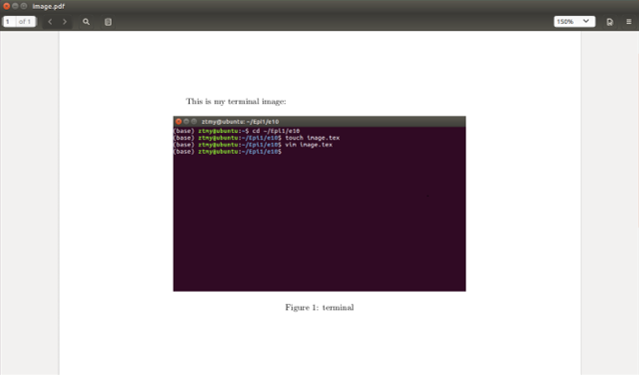
\includegraphics[width=6.65694in,height=3.91042in]{media/media/image16.png}

\textbf{五、解题感悟}

1. 学会了使用 `graphicx` 宏包和 `\textbackslash includegraphics` 命令在
LaTeX 中插入图片。

2. 了解了 `figure`、`\textbackslash centering` 和
`\textbackslash caption`
的基本作用，可以对插入的图片进行简单的排版和添加标题。

3. 通过实际编译发现，图片文件的位置和文件名需要与 LaTeX
文件对应，否则编译时容易出现找不到图片的问题。

\textbf{练习11：LaTeX 数学公式的编写}

\textbf{一、主题}

LaTeX 文档编辑

\textbf{二、题目要求}

撰写代码来生成下列公式：

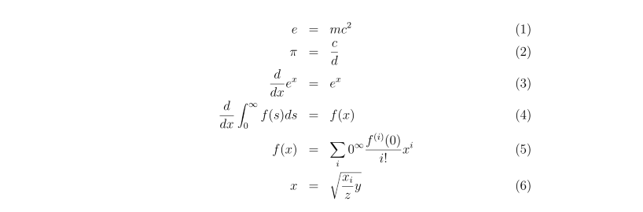
\includegraphics[width=6.69306in,height=2.21042in]{media/media/image17.png}

\textbf{三、源程序代码}

cd \textasciitilde/Epi1/e11

touch formula.tex

vim formula.tex

latexmk -pdf formula.tex

xdg-open formula.pdf

\textbf{\ul{formula.tex}}

\textbackslash documentclass\{article\}

\textbackslash begin\{document\}

\textbackslash begin\{equation\}

e = mc\^{}2

\textbackslash end\{equation\}

\textbackslash begin\{equation\}

\textbackslash pi = \textbackslash frac\{c\}\{d\}

\textbackslash end\{equation\}

\textbackslash begin\{equation\}

\textbackslash frac\{d\}\{dx\}e\^{}x = e\^{}x

\textbackslash end\{equation\}

\textbackslash begin\{equation\}

\textbackslash frac\{d\}\{dx\}\textbackslash int\_0\^{}\textbackslash infty
f(s)\textbackslash,ds = f(x)

\textbackslash end\{equation\}

\textbackslash begin\{equation\}

f(x) = \textbackslash sum\_i\^{}\textbackslash infty
\textbackslash frac\{f\^{}\{(i)\}(0)\}\{i!\}x\^{}i

\textbackslash end\{equation\}

\textbackslash begin\{equation\}

x = \textbackslash sqrt\{\textbackslash frac\{x\_i\}\{z\}y\}

\textbackslash end\{equation\}

\textbackslash end\{document\}

\textbf{四、程序运行结果}

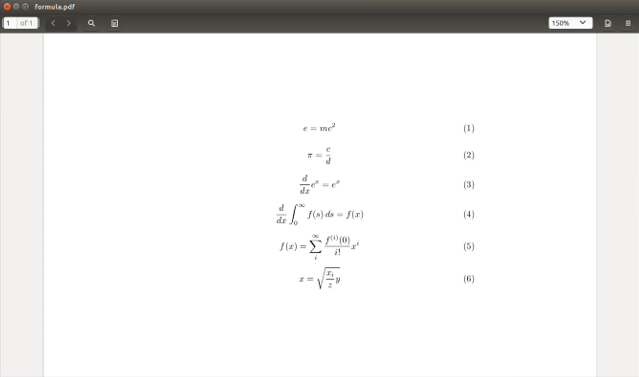
\includegraphics[width=6.65694in,height=3.92569in]{media/media/image18.png}

\textbf{五、解题感悟}

1. 学会了使用 `equation` 环境编写数学公式，并了解了公式编号的生成方式。

2. 熟悉了
`\textbackslash frac`、`\textbackslash sqrt`、`\textbackslash sum`
以及上下标等常用数学公式命令。

3. 通过实际编写不同形式的公式，对 LaTeX
数学公式的基本语法有了更深入的了解。

\end{document}
